\chapter{Organizzazione del progetto}	
		
		\section{Organizzazione strutturale}
		\label{sec:struc}
		
		La struttura organizzativa del progetto risulta difficile da stabilire in questa fase preliminare. In fasi più avanzate, i team member potranno essere suddivisi in team dedicati ad attività specifiche (Es. team di implementazione, team di testing).
		
		\begin{figure}
		\centering
		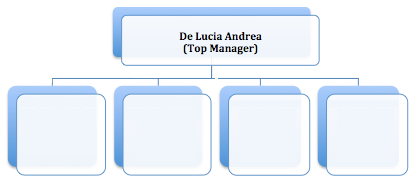
\includegraphics{img/organizzazione.png}
		\caption{Struttura organizzativa}\label{fig:1}
		\end{figure}
		
		
		\section{Ruoli e responsabilità}
		La tabella 3 riporta i componenti del team, i ruoli ad essi assegnati e le responsabilità all'interno del progetto
		
		\begin{table}[H]
			\begin{longtable}{|p{4cm}|p{4cm}|p{7cm}|}
				\hline
				Nome componente & Ruolo & Responsabilità\\
				\hline
				Matteo Merola & Project Manager & Responsabile unico della valutazione, pianificazione, realizzazione e controllo del progetto.\\[50pt]
				\hline
				Simone Scalabrino & Team member & Sviluppo deliverables: DL1 - DL3 etc\\[50pt]
				\hline
				Giovanni Grano & Team member & Sviluppo deliverables: DL1 - DL3 etc\\[50pt]
				\hline
				Carlo Branca & Team member & Sviluppo deliverables: DL1 - DL3 etc \\[50pt]
				\hline
			\end{longtable}
		\caption{Ruoli e responsabilità}\label{tab:3}
		\end {table}
		